\documentclass{bmstu}

\bibliography{biblio}

\begin{document}

\makereporttitle
    {Информатика и системы управления}
    {Программное обеспечение ЭВМ и информационные технологии}
    {лабораторной работе №~2}
    {Анализ алгоритмов}
    {}
    {}
    {Новиков~А.~А./ИУ7-52Б}
    {Строганов~Д.~В.}

\renewcommand{\contentsname}{СОДЕРЖАНИЕ} 
\tableofcontents
\setcounter{page}{2}

\begin{center}
    \textbf{ВВЕДЕНИЕ}
\end{center}
\addcontentsline{toc}{chapter}{ВВЕДЕНИЕ}

Задача коммивояжера --- одна из самых известных и старейших задач комбинаторной оптимизации. Ее корни уходят в 1831 год, когда в Германии была опубликована книга под названием "Кто такой коммивояжер и что он должен делать для процветания своего предприятия". В книге содержалась рекомендация: "Следует стремиться посетить как можно больше торговых точек, избегая повторного посещения". Это можно считать первым формулированием задачи коммивояжера~\cite{com_info}.

\textbf{Цель лабораторной работы} --- рассмотрение алгоритмов решения задачи коммивояжера.

Для достижения поставленной цели необходимо выполнить следующие задачи:
\begin{itemize}
    \item[---] сформулировать задачу коммивояжера;
    \item[---] рассмотреть алгоритмы решения: полным перебором, с использованием муравьиного алгоритма;
    \item[---] реализовать данные алгоритмы;
    \item[---] провести сравнительный анализ времени работы алгоритмов;
    \item[---] выполнить параметризацию для муравьиного алгоритма.
\end{itemize}
\chapter{Аналитический раздел}

В данном разделе будет сформулирована задача коммивояжера, а также будут рассмотрены 2 метода решения этой задачи: муравьиный алгоритм и алгоритм
полного перебора.

\section{Формулировка задачи коммивояжера}

Пусть задан граф $G = (V, E)$, где $V$ --- множество вершин ($|V|=n$), а $E$ --- множество рeбер ($|E|=m$). Каждое ребро ($(i,j)\in E$ имеет длину $c_{ij}$, определяемую матрицей расстояний $C=||c_{ij}||$. Если между вершинами $i$ и $j$ отсутствует ребро, соответствующий элемент матрицы принимается равным бесконечности ($c_{ij} = \infty$)~\cite{com_info}.

Подмножество попарно несмежных ребер графа $G$ называется паросочетанием. Паросочетание считается совершенным, если каждая вершина графа инцидентна ровно одному ребру из этого множества. Совокупность простых попарно непересекающихся циклов, покрывающая все вершины графа $G$, называется 2-фактором. Если 2-фактор состоит из одного цикла, то он называется гамильтоновым циклом~\cite{gamelton}.

Задача заключается в поиске гамильтонова цикла минимальной длины, то есть цикла, который проходит через каждую вершину графа ровно один раз и возвращается в начальную точку.


\subsection{Алгоритм полного перебора}
Алгоритм полного перебора для решения задачи коммивояжера основывается на проверке всех возможных маршрутов в графе для определения минимального. Этот метод заключается в полном переборе всех вариантов обхода городов и выборе маршрута с наименьшей длиной. Однако количество возможных маршрутов быстро растет с увеличением числа городов $n$, поскольку сложность алгоритма составляет $n!$. Несмотря на то, что данный подход гарантирует получение точного решения, его применение становится крайне неэффективным даже при относительно небольшом количестве городов из-за значительных вычислительных затрат.

\subsection{Муравьиный алгоритм}
В основе муравьиного алгоритма лежит идея моделирования поведения колонии муравьев. Каждый муравей определяет свой маршрут на основе оставленных другими муравьями феромонов, а также сам оставляет оставляет феромоны, чтобы последующие муравьи ориентировались по ним. В результате при прохождении каждым муравьем своего маршрута наибольшее число феромонов остается на самом оптимальном пути. Временная сложность алгоритма была оценена как $683 - (42,467 · N) + (1,0696 · N^2)$~\cite{ants}. Однако главный недостаток алгоритма заключается в том, что, по сравнению с алгоритмом полного перебора, он дает приближенное решение задачи, а не точное.

Вероятность перехода муравья $k$ из текущей вершины $i$ в вершину $j$ рассчитывается по формуле:
\begin{equation}
    \label{posib}
    P_{kij} = 
    \begin{cases}
        \frac{\tau_{ij}^a \eta_{ij}^b}{\sum_{q \in J_{ik}} \tau_{iq}^a \eta_{iq}^b}, & \text{если вершина $j$ еще не посещена муравьем $k$,} \\
        0, & \text{иначе,}
    \end{cases}
\end{equation}
где:
\begin{itemize}
    \item[---] $a$ --- параметр влияния феромона;
    \item[---] $b$ --- параметр влияния длины пути;
    \item[---] $\tau_{ij}$ --- количество феромонов на ребре $(i, j)$;
    \item[---] $\eta_{ij}$ --- видимость (величина обратная расстоянию до вершины).
\end{itemize}

По окончанию движения всех муравьев уровень феромонов на ребрах обновляется по формуле:
\begin{equation}
    \label{update_phero_1}
    \tau_{ij}(t+1) = (1-p)\tau_{ij}(t) + \Delta \tau_{ij},
\end{equation}

где $p$ — коэффициент испарения феромона, а $\Delta \tau_{ij}$ определяется как:

\begin{equation}
    \label{update_phero_2}
    \Delta \tau_{ij} = \sum_{k=1}^N \Delta \tau_{ij}^k,
\end{equation}

\begin{equation}
    \label{update_phero_3}
    \Delta \tau_{ij}^k = 
    \begin{cases}
        \frac{Q}{L_k}, & \text{если ребро $(i, j)$ посещено муравьем $k$,} \\
        0, & \text{иначе,}
    \end{cases}
\end{equation}

где $Q$ — параметр, связанный с длиной оптимального пути, а $L_k$ — длина маршрута муравья $k$.

\subsection{Описание алгоритма}
Пошаговое описание муравьиного алгоритма:
\begin{enumerate}
    \item[1)] Муравей исключает из дальнейшего выбора вершины, которые уже были посещены, ссылаясь на список посещенных вершин, хранящийся в его памяти (список запретов $J_{ik}$).
    \item[2)] Муравей оценивает привлекательность вершин, основываясь на их видимости, которая обратно пропорциональна расстоянию между ними.
    \item[3)] Муравей ощущает уровень феромонов на ребрах графа, что помогает ему определять предпочтительность маршрута.
    \item[4)] После прохождения ребра $(i, j)$ муравей оставляет на нем феромоны, количество которых зависит от длины маршрута $L_k$, пройденного муравьем, и параметра $Q$.
\end{enumerate}

\textbf{ВЫВОД}

В данном разделе была представлена формулировка задача коммивояжера, а также рассмотрены 2 метода ее решения: муравьиный алгоритм и алгоритм полного перебора

\chapter{Конструкторский раздел}
В данном разделе будут определены требования к программному обеспечению
и приведены схемы алгоритма полного перебора и муравьиного алгоритма для
решения задачи коммивояжера.

\section{Требования к программному обеспечению}
Входные данные: матрица стоимостей взвешенного неориентированного графа.

Выходные данные: кратчайший гамильтонов цикл.

\section{Представления алгоритмов}
На рисунках~\ref{fig:brute_force}~---~\ref{fig:ant} представлены схема алгоритма полного перебора и схема муравьиного алгоритма.

\begin{figure}[H]
    \centering
    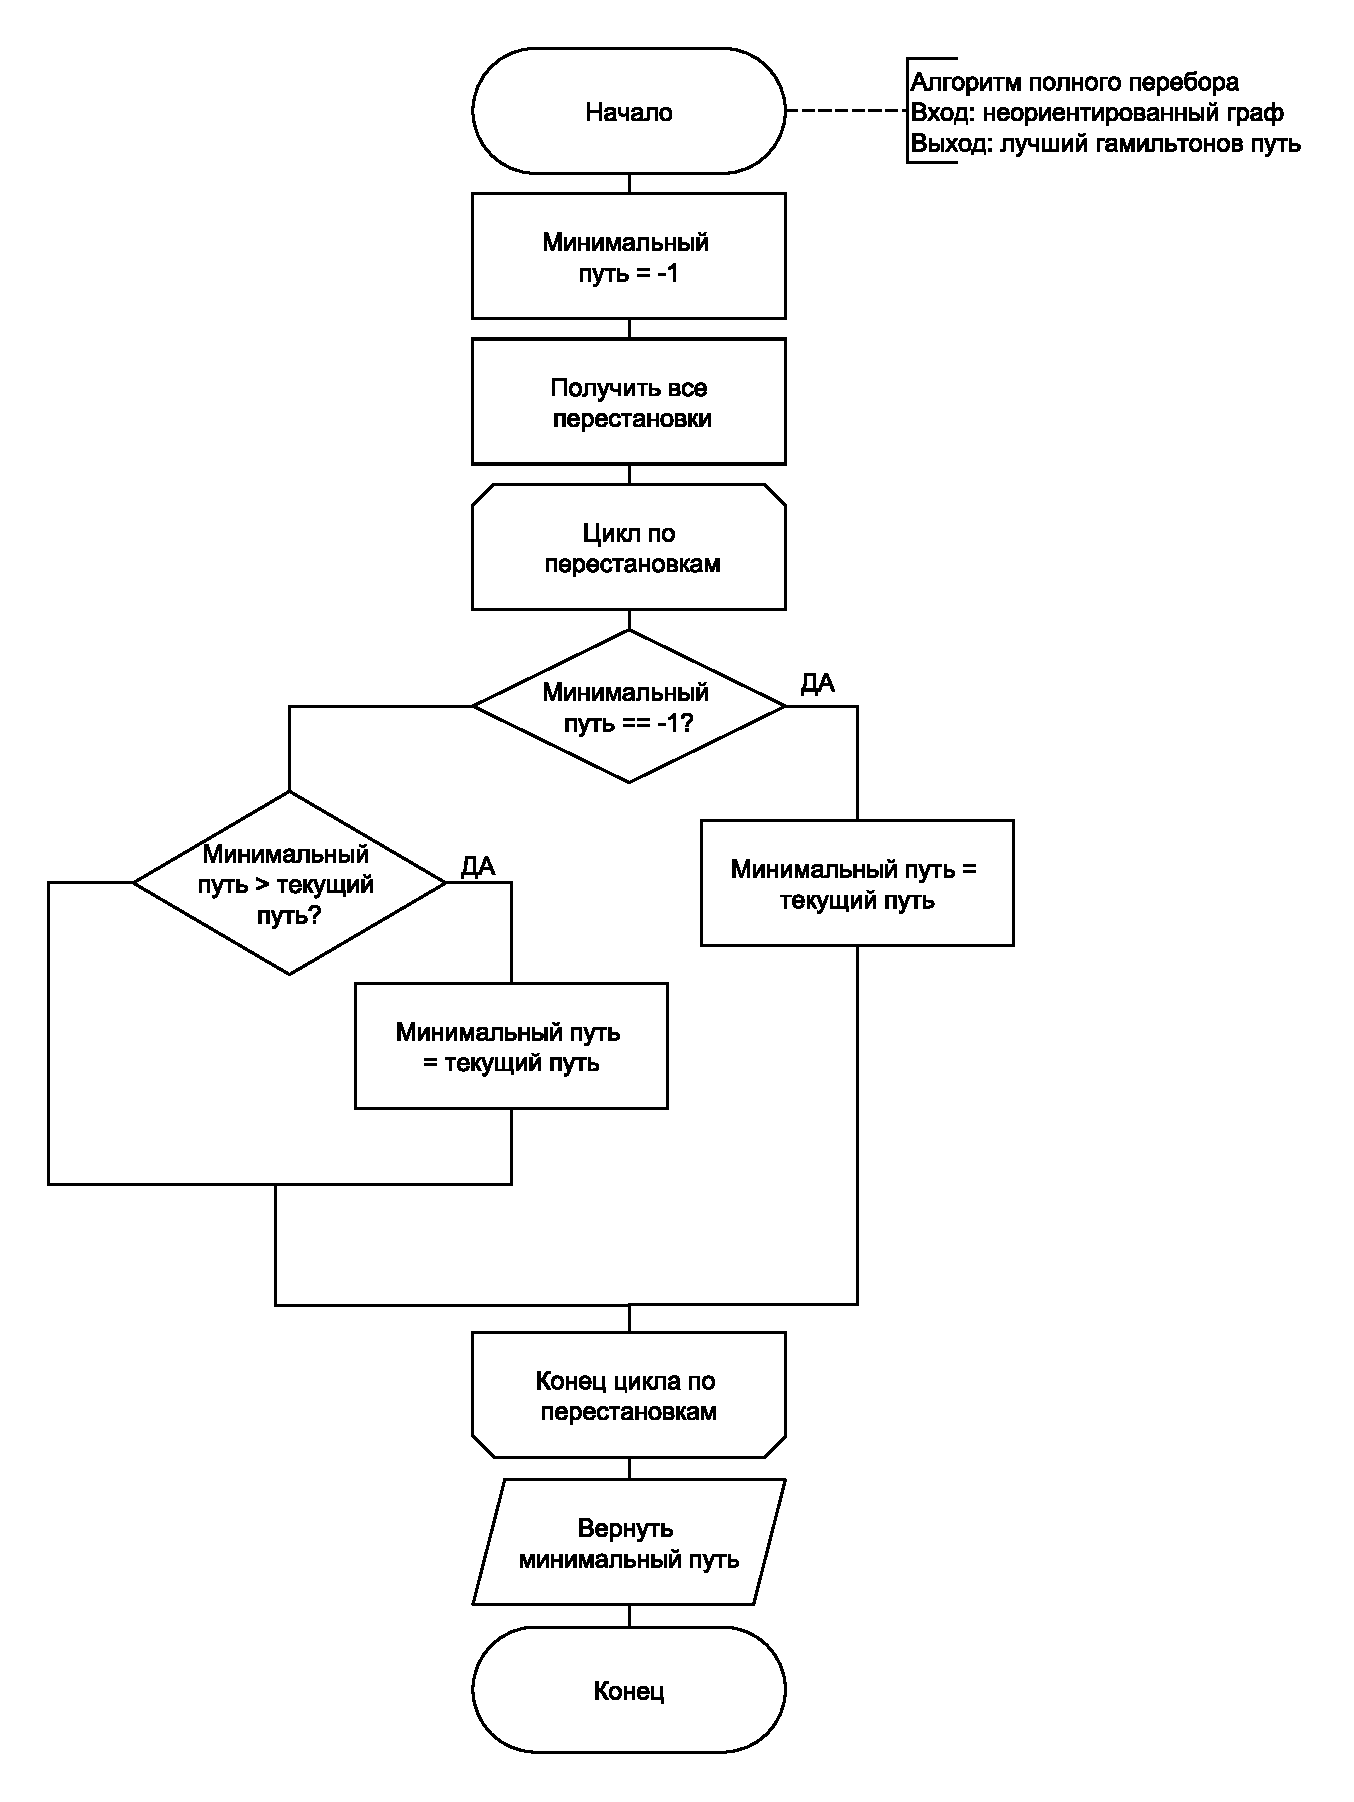
\includegraphics[scale=0.7]{img/unnamed1.eps}
    \caption{Схема алгоритма полного перебора}
    \label{fig:brute_force}
\end{figure}

\begin{figure}[H]
    \centering
    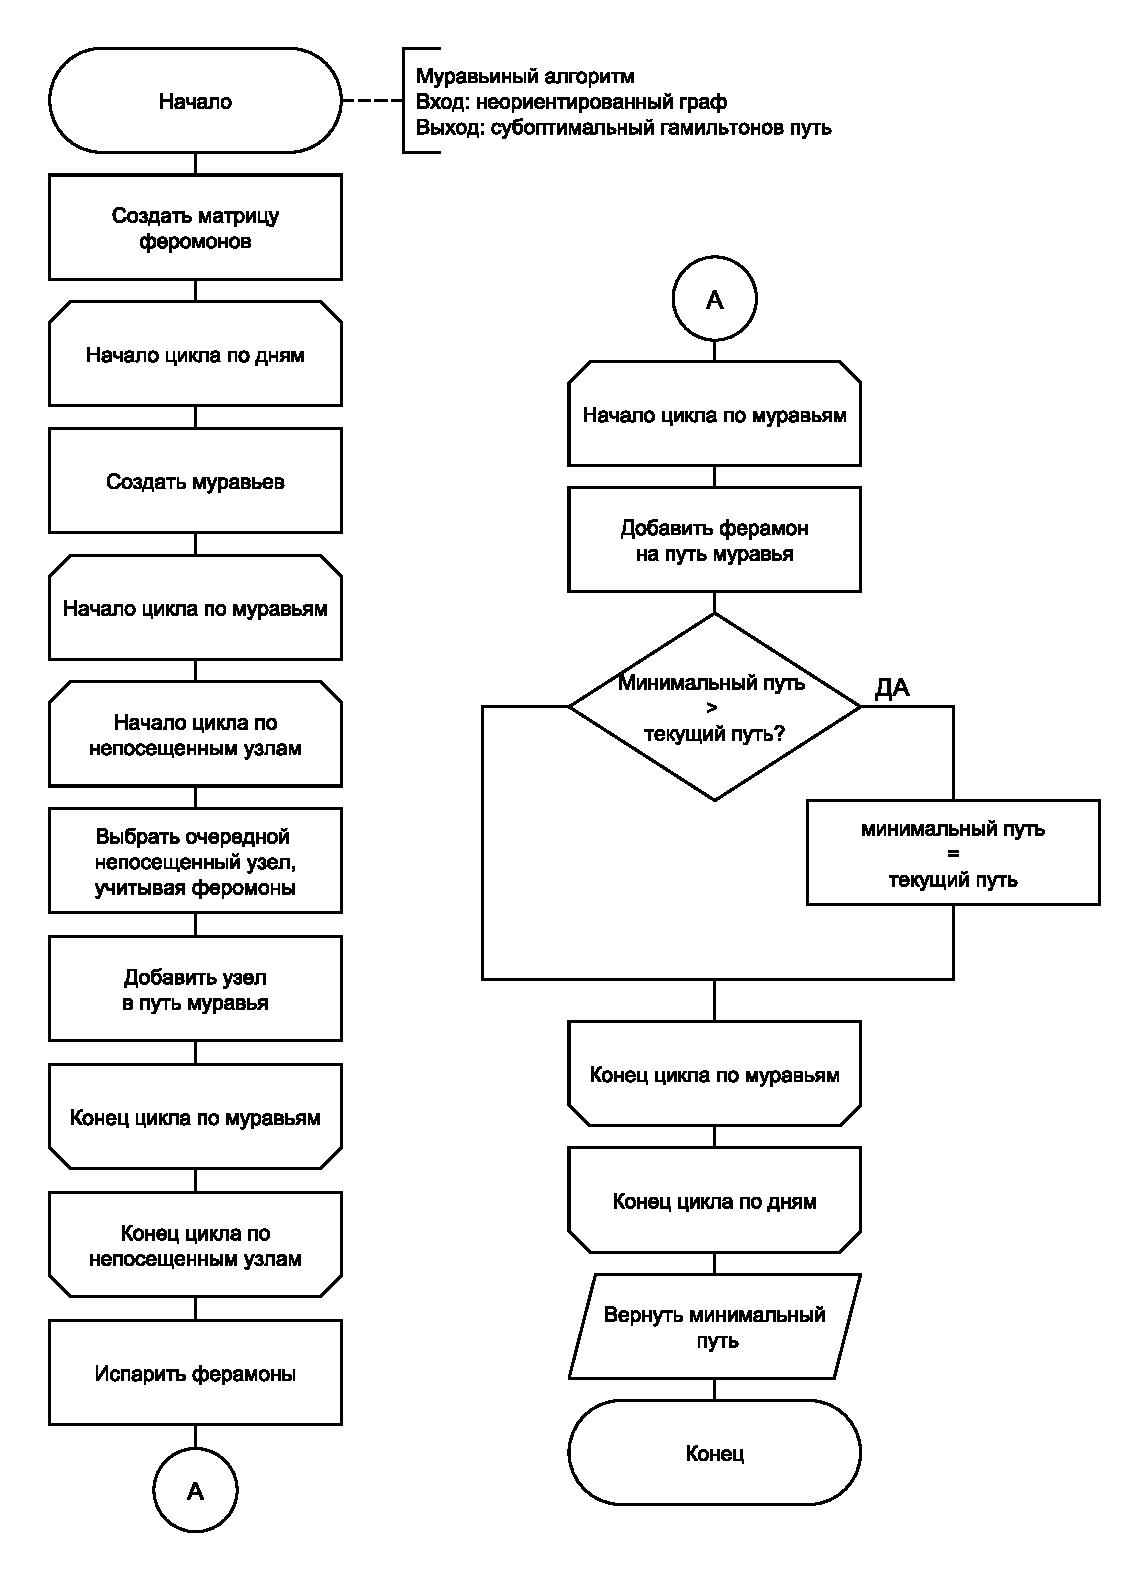
\includegraphics[scale=0.7]{img/unnamed2.eps}
    \caption{Схема муравьиного алгоритма}
    \label{fig:ant}
\end{figure}

\textbf{ВЫВОД}

В данном разделе были определены требования к программному обеспечению и приведены схемы алгоритмов полного перебора и муравьиного алгоритма для решения задачи коммивояжера.

\clearpage
\chapter{Технологический раздел}

В данном разделе описаны требования к программному обеспечению, реализация алгоритмов и средства реализации.

\section{Требования к программному обеспечению}

Входные данные: массив и искомый элемент;
Выходные данные: индекс искомого элемента или значение, сигнализирующие об отсутствии искомого элемента в массиве.


\section{Средства реализации}
Для реализации данной лабораторной работы выбран язык программирования высокого уровня Python \cite{python}. Выбор был обусловлен наличием библиотеки $matplotlib$ \cite{python_matplotlib}. Для построения графиков была выбрана функция $bar$ \cite{python_matplotlib_bar}.

\section{Реализация алгоритмов}
В листингах \ref{lst:liniar} --- \ref{lst:binary} представлены представлены реализации алгоритмов.

\begin{center}
\captionsetup{justification=raggedright,singlelinecheck=off}
\begin{lstlisting}[language=Python, frame=single, numbers=left, label=lst:liniar, caption=Реализация алгоритма линейного поиска]
def linear_search(array: list, item: int) -> int | None:
    n = len(array)
    i = 0
    index = None
    
    while i < n:
        if larray[i] == item:
            index = i
            break
        i += 1
        
    return index
\end{lstlisting}
\end{center}

\clearpage

\begin{center}
\captionsetup{justification=raggedright,singlelinecheck=off}
\begin{lstlisting}[language=Python, frame=single, numbers=left, label=lst:binary,caption=Реализация алгоритма бинарного поиска]
def binary_search(array: list, item: int) -> int | None:
    left = 0
    right = len(array) - 1
    index = None
    
    while left <= right:
        mid = (left + right) // 2
        if array[mid] == item:
            item = mid
            break

        if item < array[mid]:
            right = mid - 1
        else:
            left = mid + 1

    return item

\end{lstlisting}
\end{center}

\clearpage


\clearpage

\textbf{ВЫВОД}

В данном разделе были представлены реализации алгоритмов поиска заданного элемента в массиве методом линейного поиска и методом бинарного поиска, были рассмотрены средства реализации, предъявлены требования к программному обеспечению.
\clearpage
\chapter{Исследовательский раздел}
В данном разделе проведен сравнительный анализ алгоритмов по используемому процессорному времени.

\section{Технические характеристики}
Технические характеристики используемого устройства:
\begin{itemize}
    \item[---] Операционная система --- Windows 10 Home \cite{Windows}
    \item[---] Память --- 16 Гб.
    \item[---] Процессор --- Intel(R) Core(TM) i5-10300H CPU @ 2.50 Ггц \cite{Intel}
    \item[---] Микроконтроллер --- STM32F303 \cite{STM}
\end{itemize}


\section{Время выполнения алгоритмов}
Время работы трех алгоритмов умножения матриц было измерено и представлено в таблице \ref{tbl:time_measurements}. Тестирование проводилось на микроконтроллере STM32F303 с тактовой частотой до 72 МГц. Измерения выполнялись на матрицах одинакового размера и усреднялись для каждого набора однотипных экспериментов. Каждое значение является средним результатом 100 замеров. График зависимости времени умножения от размера матриц для трех алгоритмов показан на рисунке \ref{fig:tm}.

\begin{table}[h]
	\begin{center}
		\begin{threeparttable}
		\captionsetup{justification=raggedright,singlelinecheck=off}
		\caption{Время работы алгоритмов (в мс)}
		\label{tbl:time_measurements}
		\begin{tabular}{|c|r|r|r|r|}
			\hline
			Размер матрицы & Классический & Виноград & Виноград (оптимизированный) \\
            \hline
			3    & 0.3 & 0.3 & 0.5 \\
            \hline
			5    & 1.1 & 1.5 & 1.3 \\ 
            \hline
			7    & 2.9 & 3.3 & 2.8 \\ 
            \hline
			9    & 5.7 & 6.4 & 5.7 \\ 
			\hline
			11    & 10.2 & 11.0 & 9.7 \\ 
			\hline
			13    & 18.0 & 18.3 & 16.3 \\ 
			\hline
			15    & 28.9 & 26.5 & 24.0 \\ 
			\hline
			17    & 39.6 & 38.6 & 36.6 \\ 
			\hline
			19    & 51.8 & 51.4 & 46.0 \\ 
			\hline
			21    & 68.7 & 72.7 & 61.9 \\ 
			\hline
			23    & 97.5 & 96.0 & 83.0 \\ 
			\hline
            25    & 122.3 & 114.1 & 108.0 \\ 
            \hline
            27    & 149.9 & 153.2 & 138.1 \\ 
            \hline
            29   & 180.1 & 175.3 & 161.8 \\ 
            \hline
            31   & 239.1 & 230.1 & 208.0 \\ 
            \hline
            33   & 282.9 & 282.9 & 247.4 \\ 
            \hline
            35   & 329.5 & 329.5 & 298.6 \\ 
            \hline
		\end{tabular}
		\end{threeparttable}
    \end{center}
\end{table}

\clearpage

\begin{figure}[H]
    \centering
    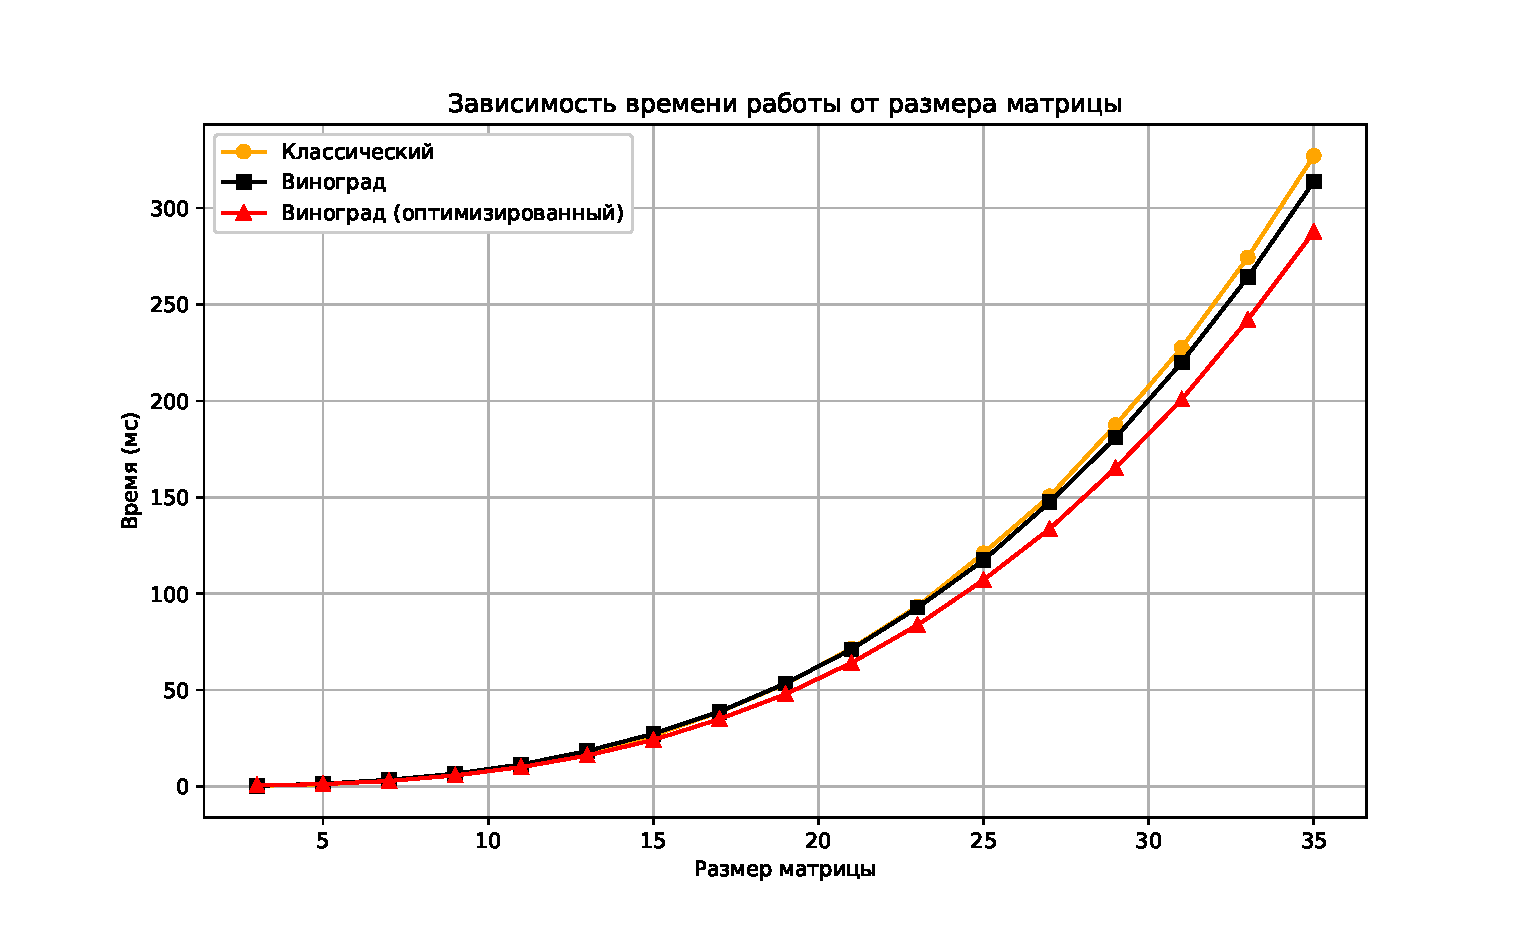
\includegraphics[width=1\linewidth]{img/graph.eps}
    \caption{Сравнение алгоритмов по времени}
    \label{fig:tm}
\end{figure}

\clearpage

\textbf{ВЫВОД}

Исследование показало, что классический алгоритм умножения матриц уступает алгоритму Винограда по скорости примерно в 1,2 раза, поскольку в алгоритме Винограда часть вычислений выполняется заранее, а количество сложных операций, таких как умножение, уменьшается. Следовательно, алгоритм Винограда предпочтительнее. Оптимизированный алгоритм Винограда, в свою очередь, демонстрирует еще лучшее время работы — он быстрее на 1,2 раза на матрицах размером более 10 элементов благодаря замене операций сложения и присваивания, сдвигу вместо умножения и предварительным вычислениям некоторых выражений. Таким образом, для наилучшей производительности стоит выбирать оптимизированный алгоритм Винограда.

Кроме того, выявлено, что на матрицах с четным размером алгоритм Винограда работает быстрее, чем на нечетных, что связано с необходимостью дополнительной обработки крайних строк и столбцов. Соответственно, алгоритм Винограда наиболее эффективен для матриц с четными размерами.
\begin{center}
    \textbf{ЗАКЛЮЧЕНИЕ}
\end{center}
\addcontentsline{toc}{chapter}{ЗАКЛЮЧЕНИЕ}

Экспериментально были выявлены различия между алгоритмами линейного поиска и бинарного поиска при поиске заданного элемента в множестве с использованием специально разработанного программного обеспечения.

Исследования подтвердили, что алгоритм полного перебора уступает бинарному поиску по числу сравнений, необходимых для нахождения элемента в массиве.

\vspace{5mm}

В ходе выполнения данной лабораторной работы были решены следующие задачи:
\begin{itemize}
    \item[---] реализованы алгоритмы нахождения заданного значения в массиве методом линейного поиска и методом бинарного поиска;
    \item[---] проанализированы реализации алгоритмов по количеству сравнений для нахождения каждого элемента;
    \item[---] описаны полученные результаты в отчете.
\end{itemize}
\makebibliography



\end{document}